%%%%%%%%%%%%%%%%%%%%%%%%%%%%%%%%%%%%%%%%%%%%%%%%%%%%%%%%%%%%%%%%%%%%%%%%%%%%%%%%%%%%%%%%%%
\section{Results}

%%%%%%%%%%%%%%% Parameters %%%%%%%%%%%%%%%
% n_data = 20 - n_data in x and y: n_tot = 20*20
% test_size = 0.2
% noise = 0.2 - aptitude of normal distributed noise    
% data_dim = 2

%%%%%%%%%%%%%%% Part b %%%%%%%%%%%%%%%
% * Evaluate MSE up to 5.th order fro OLS. 
% * and R2 score
% * blot parameters beta
% * Your code has to include a scaling/centering:
%   XXX: not included, data is already scaled in intervall [-1, 1]

\begin{figure}[H]
    \centering
    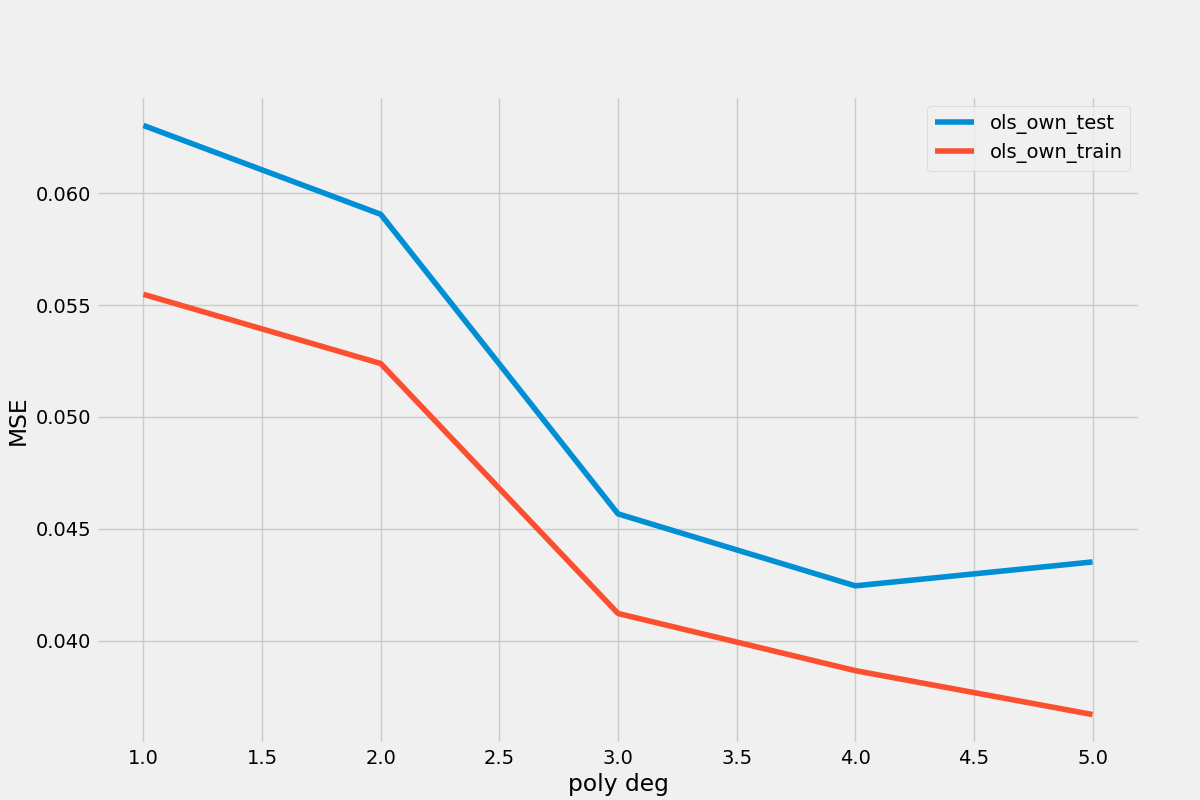
\includegraphics[width=0.8\textwidth]{Figures/b_mse.png}
\end{figure}

\begin{figure}[H]
    \centering
    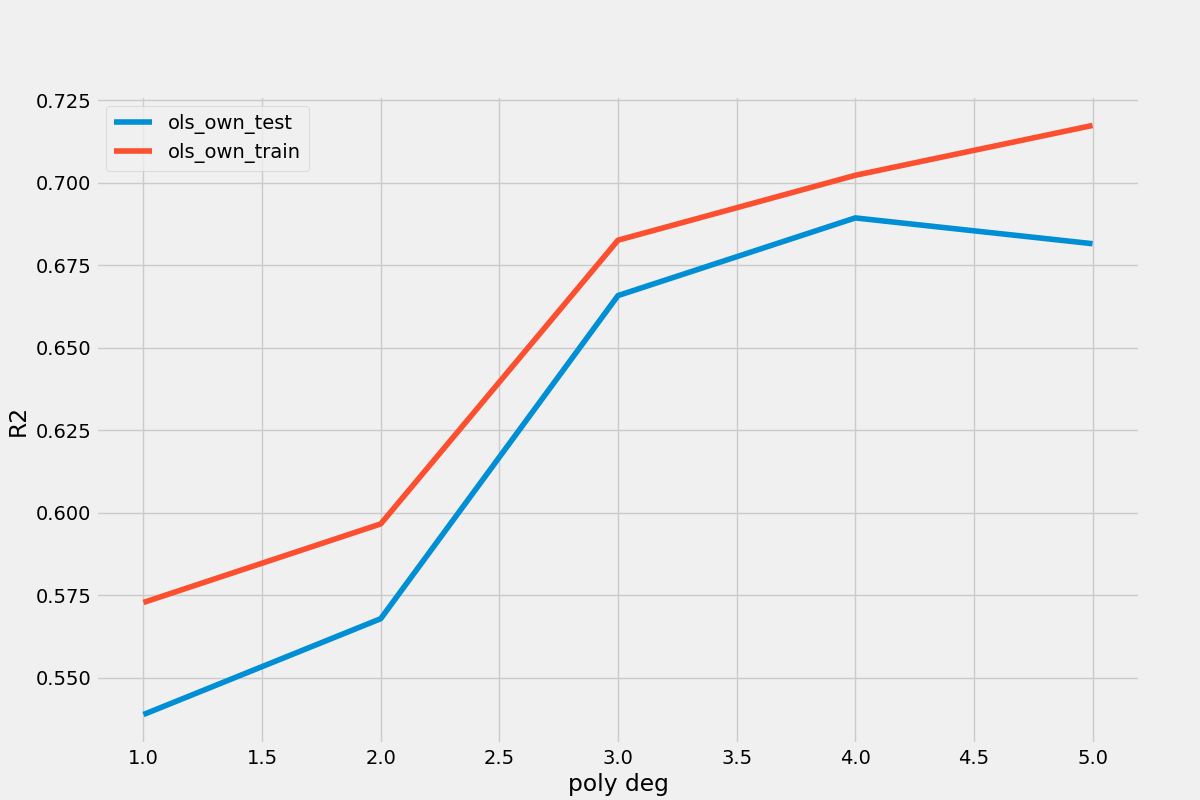
\includegraphics[width=0.8\textwidth]{Figures/b_r2.png}
\end{figure}

% TODO: error bars
\begin{figure}[H]
    \centering
    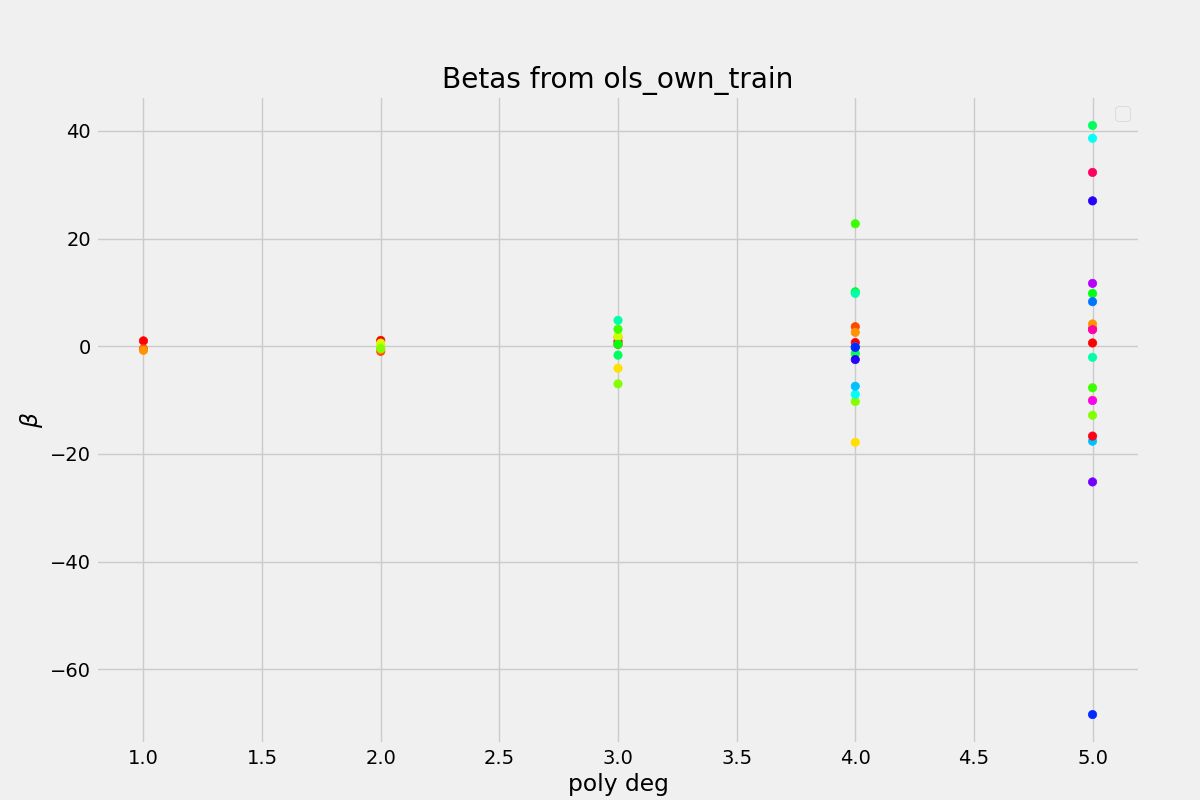
\includegraphics[width=0.8\textwidth]{Figures/b_beta.png}
\end{figure}

%For bootstrap: should consider plotting a histogram of the estimators beta_hat^* as this should resemble a pdf. 

%%%%%%%%%%%%%%% Part c  %%%%%%%%%%%%%%%
% * Explain bias, variance, mse terms (theory) and interpretation 
% * Bias variance analysis on franke function
% * discuss in bias variance trade-off in terms of:
%   * model complexity
%   * number of data points
%   * training and test data


\begin{figure}[H]
    \centering
    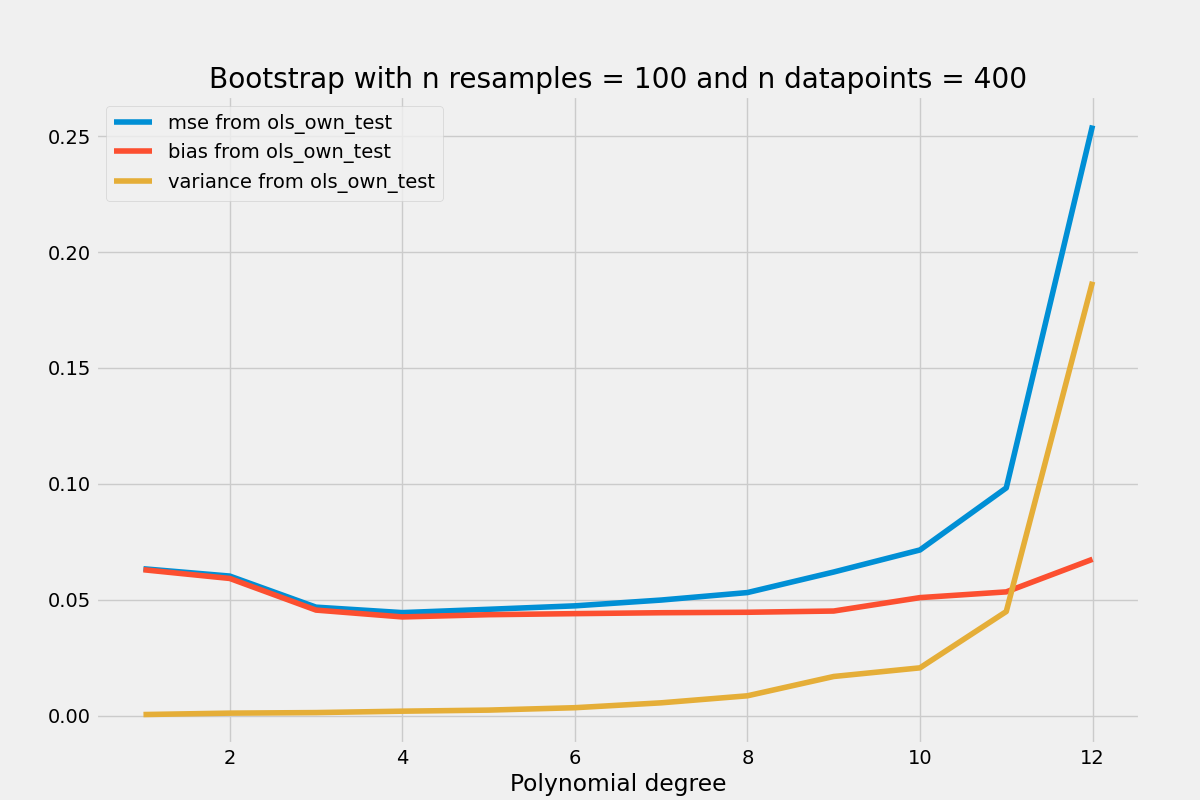
\includegraphics[width=0.8\textwidth]{Figures/c_bootstrap_ols_n_data_400.png}
\end{figure}


\begin{figure}[H]
    \centering
    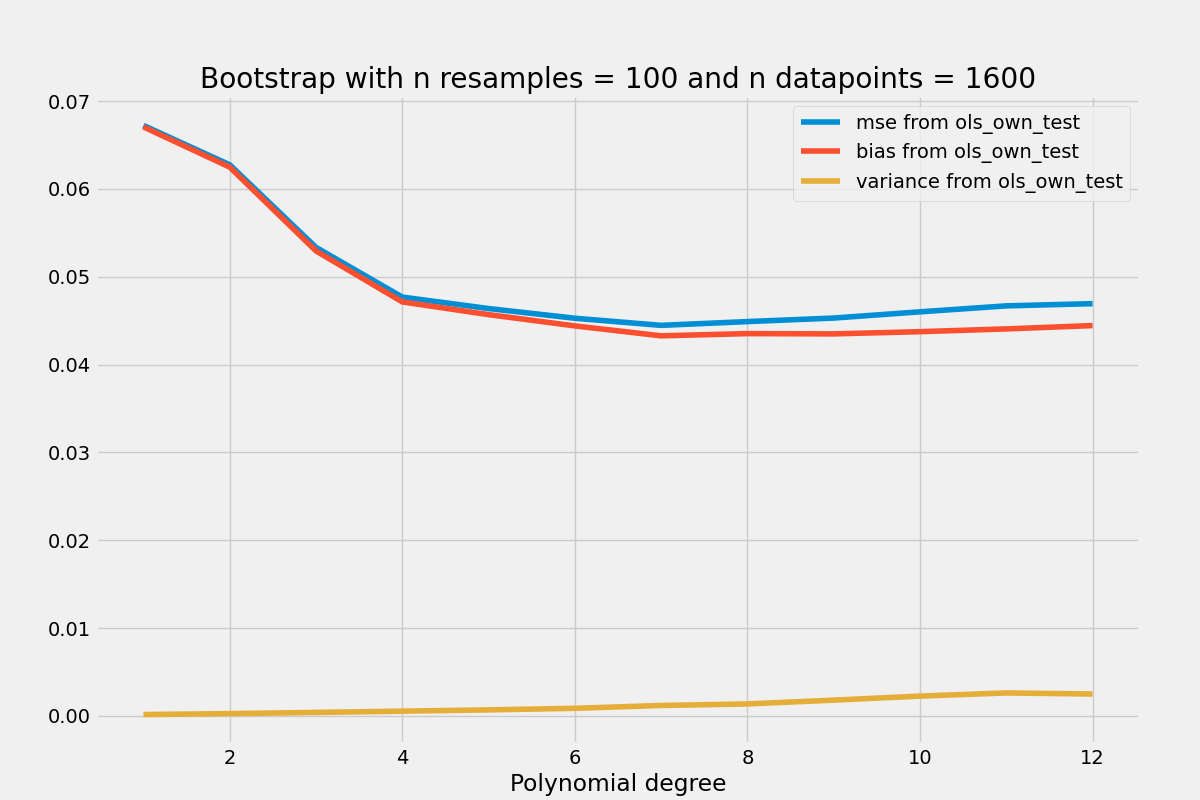
\includegraphics[width=0.8\textwidth]{Figures/c_bootstrap_ols_n_data_1600.png}
\end{figure}

% XXX: Is this expected behaviour?
\begin{figure}[H]
    \centering
    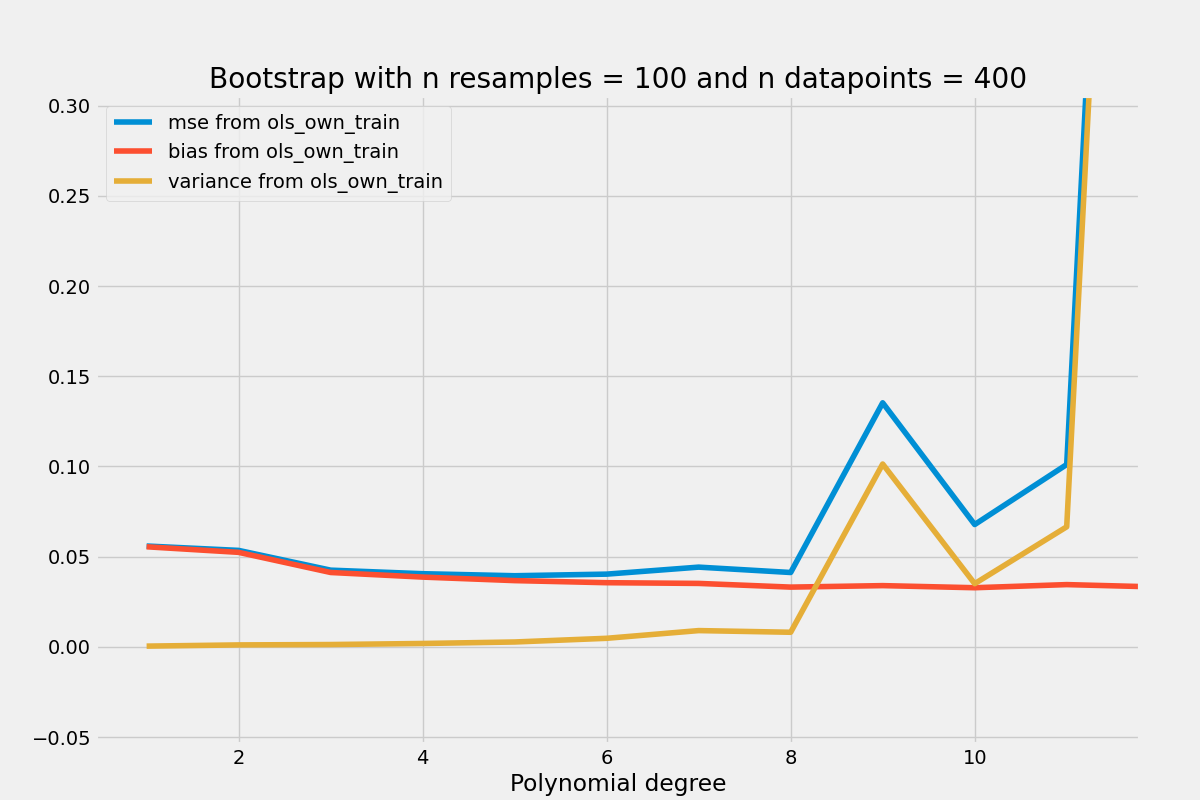
\includegraphics[width=0.8\textwidth]{Figures/c_bootstrap_ols_n_data_400_train_data.png}
\end{figure}

%%%%%%%%%%%%%%% Part d %%%%%%%%%%%%%%%
% Use k-fold and evaluate MEE on test data
% compare with bootstrap
% compare with sklearn

\begin{figure}[H]
    \centering
    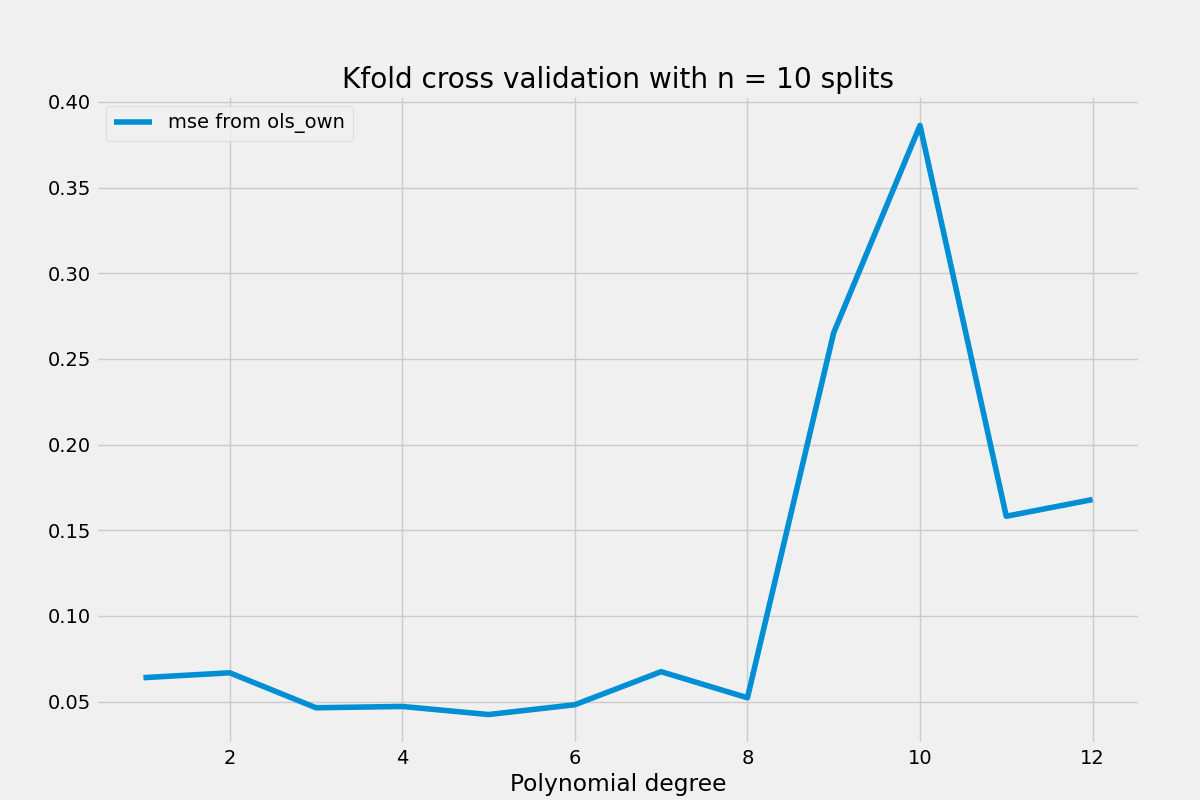
\includegraphics[width=0.8\textwidth]{Figures/d_kfold_ols_n_10.png}
\end{figure}

%%%%%%%%%%%%%%% Part e %%%%%%%%%%%%%%%
% * bootstrap analysis for ridge as in part c
% * and cross validation as in part d 
% * Compare results to those obtained in part b-d
% * study bias variance trade off for different values of lambda 

The minimum MSE from Ridge regression was found for polynomial degree of 6 with
the hyper parameter, $\lambda = 0.001$
\begin{figure}[H]
    \centering
    \caption{ridge}  
    \label{fig:e_ridge} 
    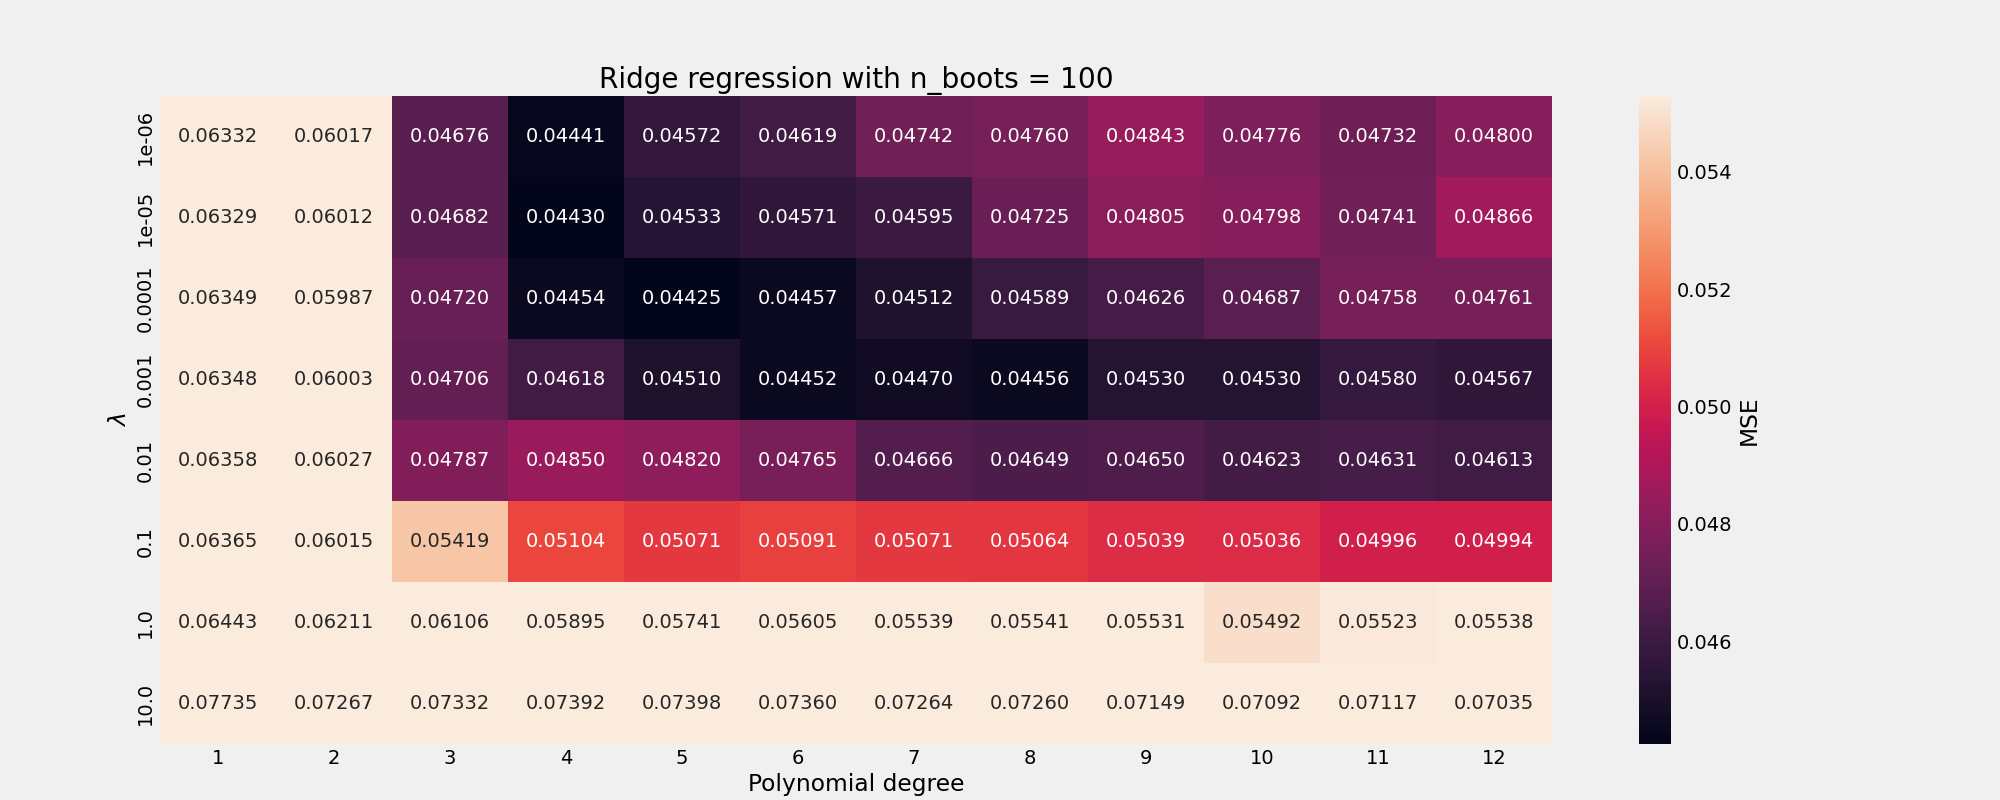
\includegraphics[width=1\textwidth]{Figures/e_ridge_n_boots_100.png}
\end{figure}

\begin{figure}[H]
    \centering
    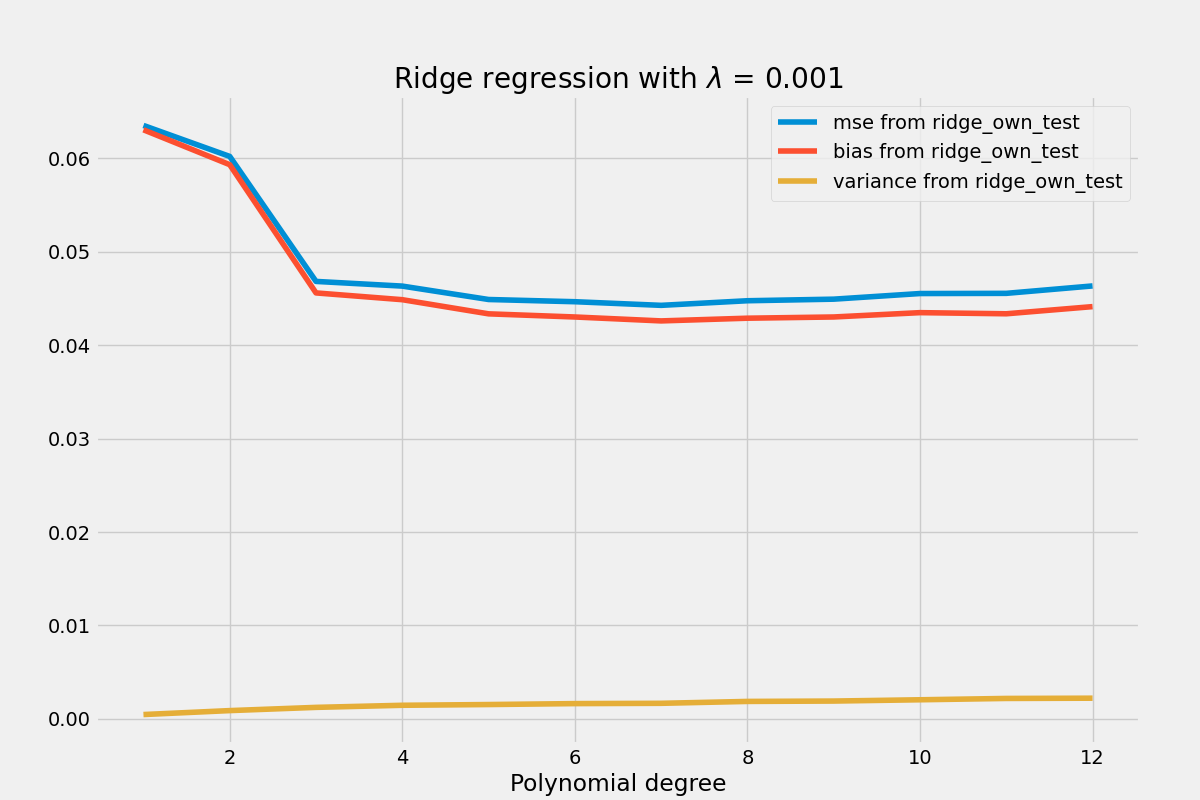
\includegraphics[width=0.8\textwidth]{Figures/e_ridge_bias_variance_lamb_0_001.png}
\end{figure}


\begin{figure}[H]
    \centering
    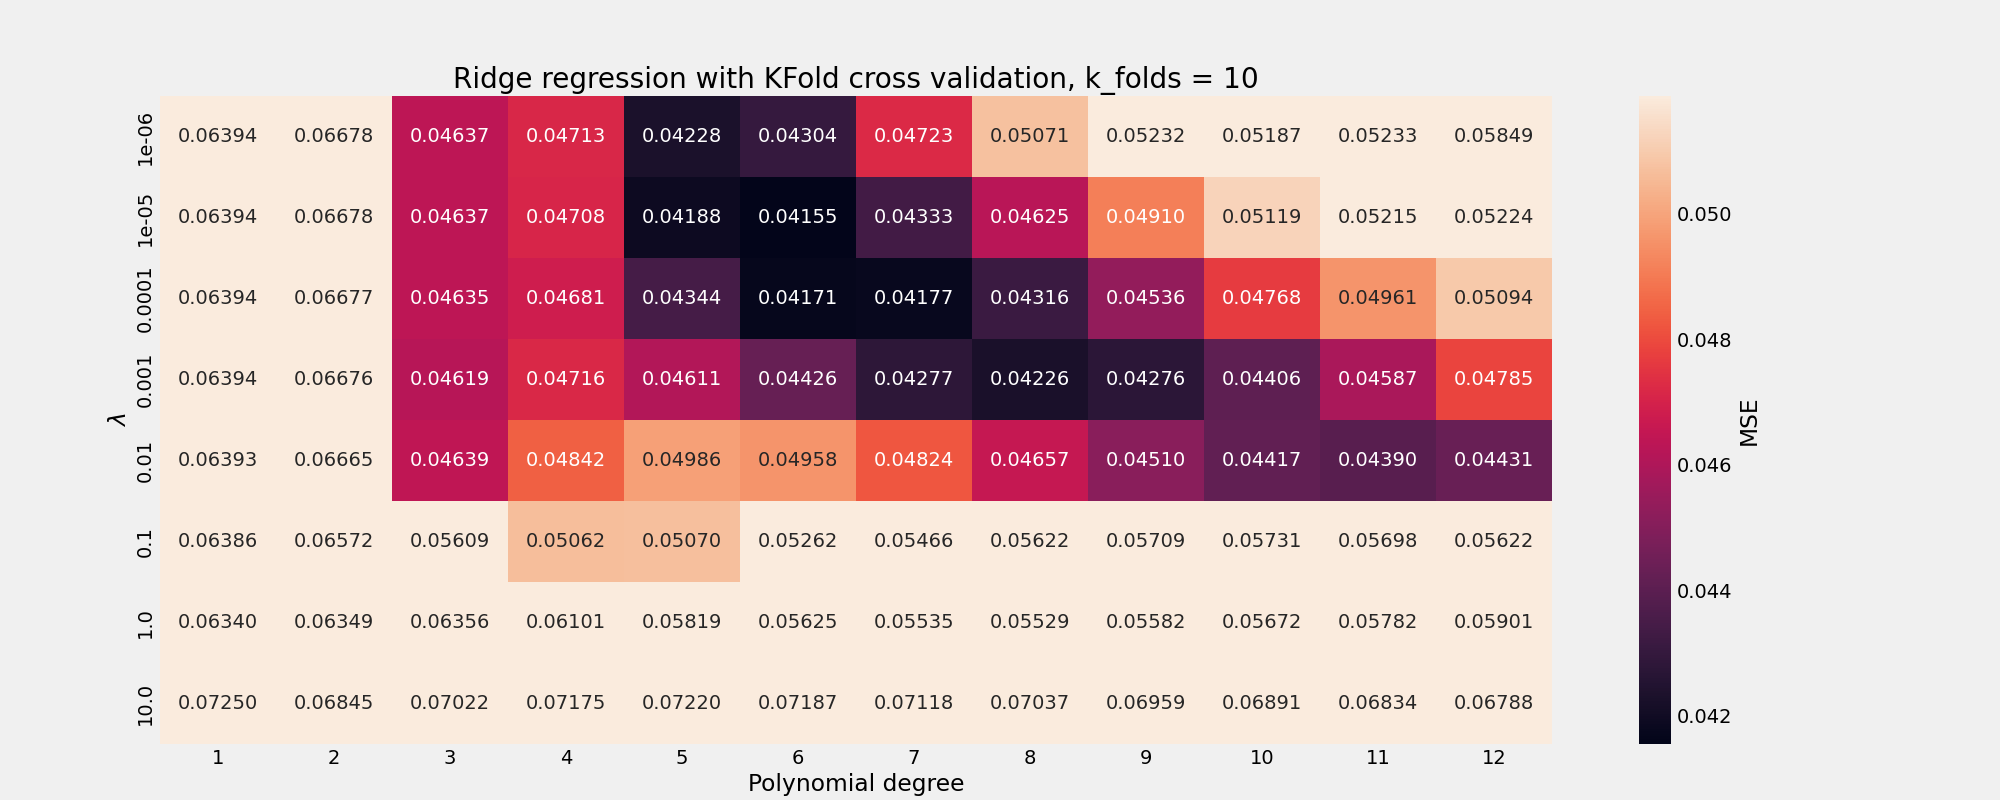
\includegraphics[width=0.8\textwidth]{Figures/e_ridge_kfold_n_10.png}
\end{figure}

%%%%%%%%%%%%%%% Part f %%%%%%%%%%%%%%%
% * Lasso regression
% * give a critical discussion of mse, ridge, lasso
% * Which model fits the data best 
% * bootstrap bias variance analysis of lasso
% * MSE analysis with kfold


\begin{figure}[H]
    \centering
    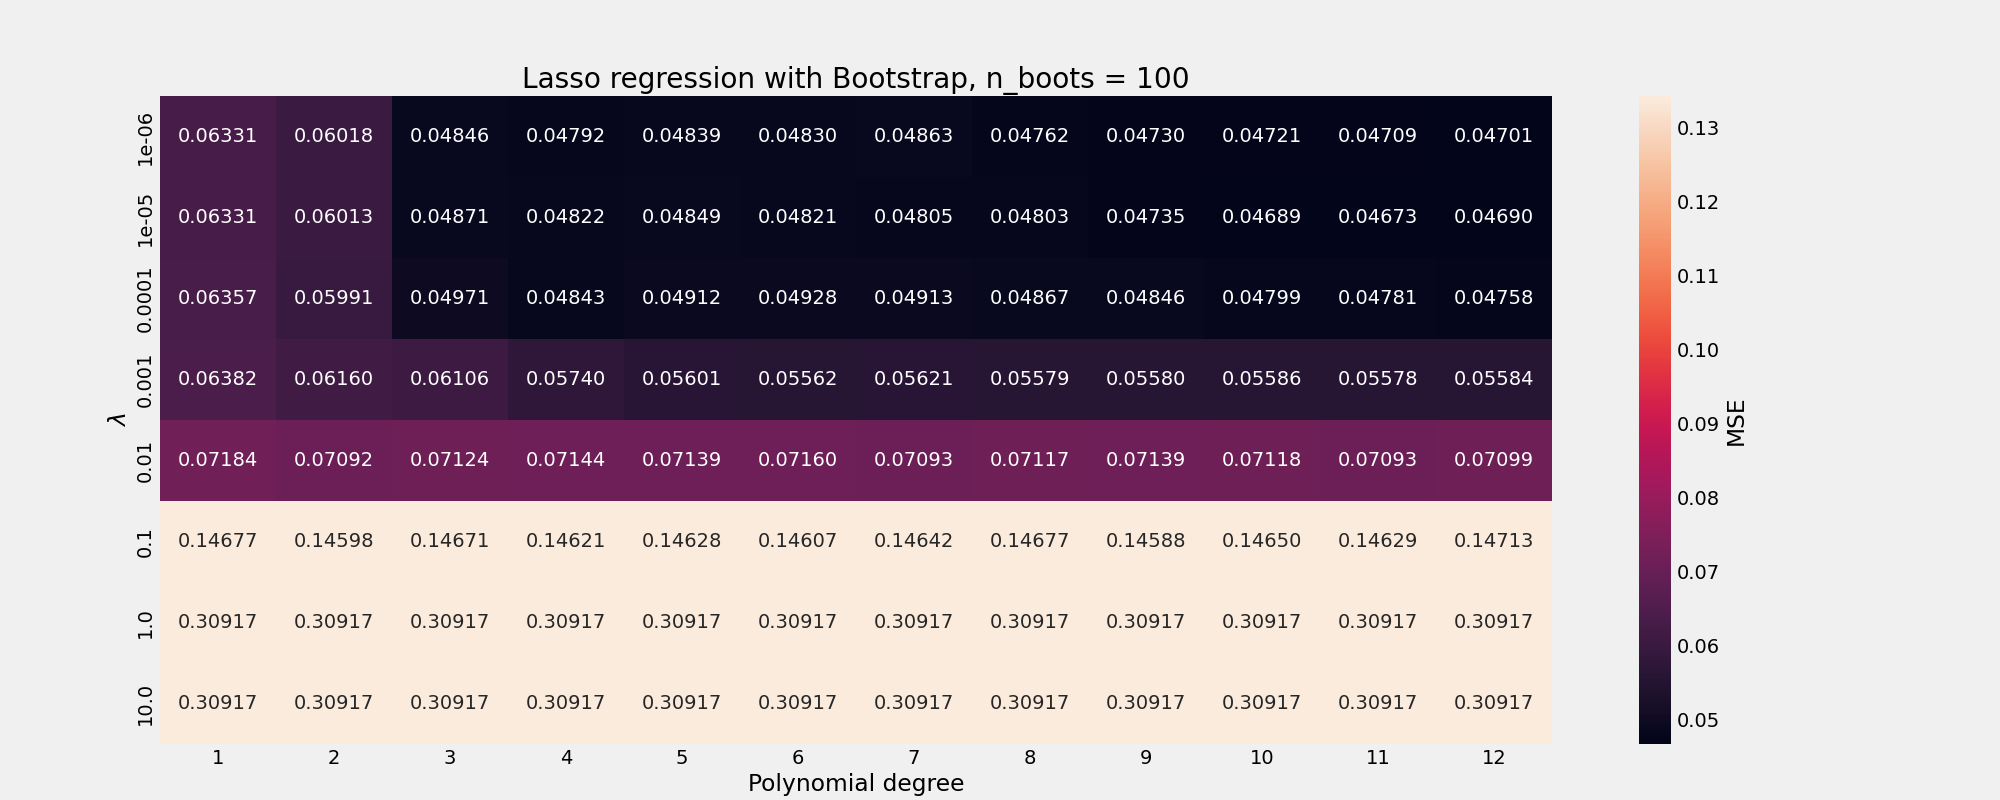
\includegraphics[width=0.8\textwidth]{Figures/f_lasso_bootstrap_n_100.png}
\end{figure}

\begin{figure}[H]
    \centering
    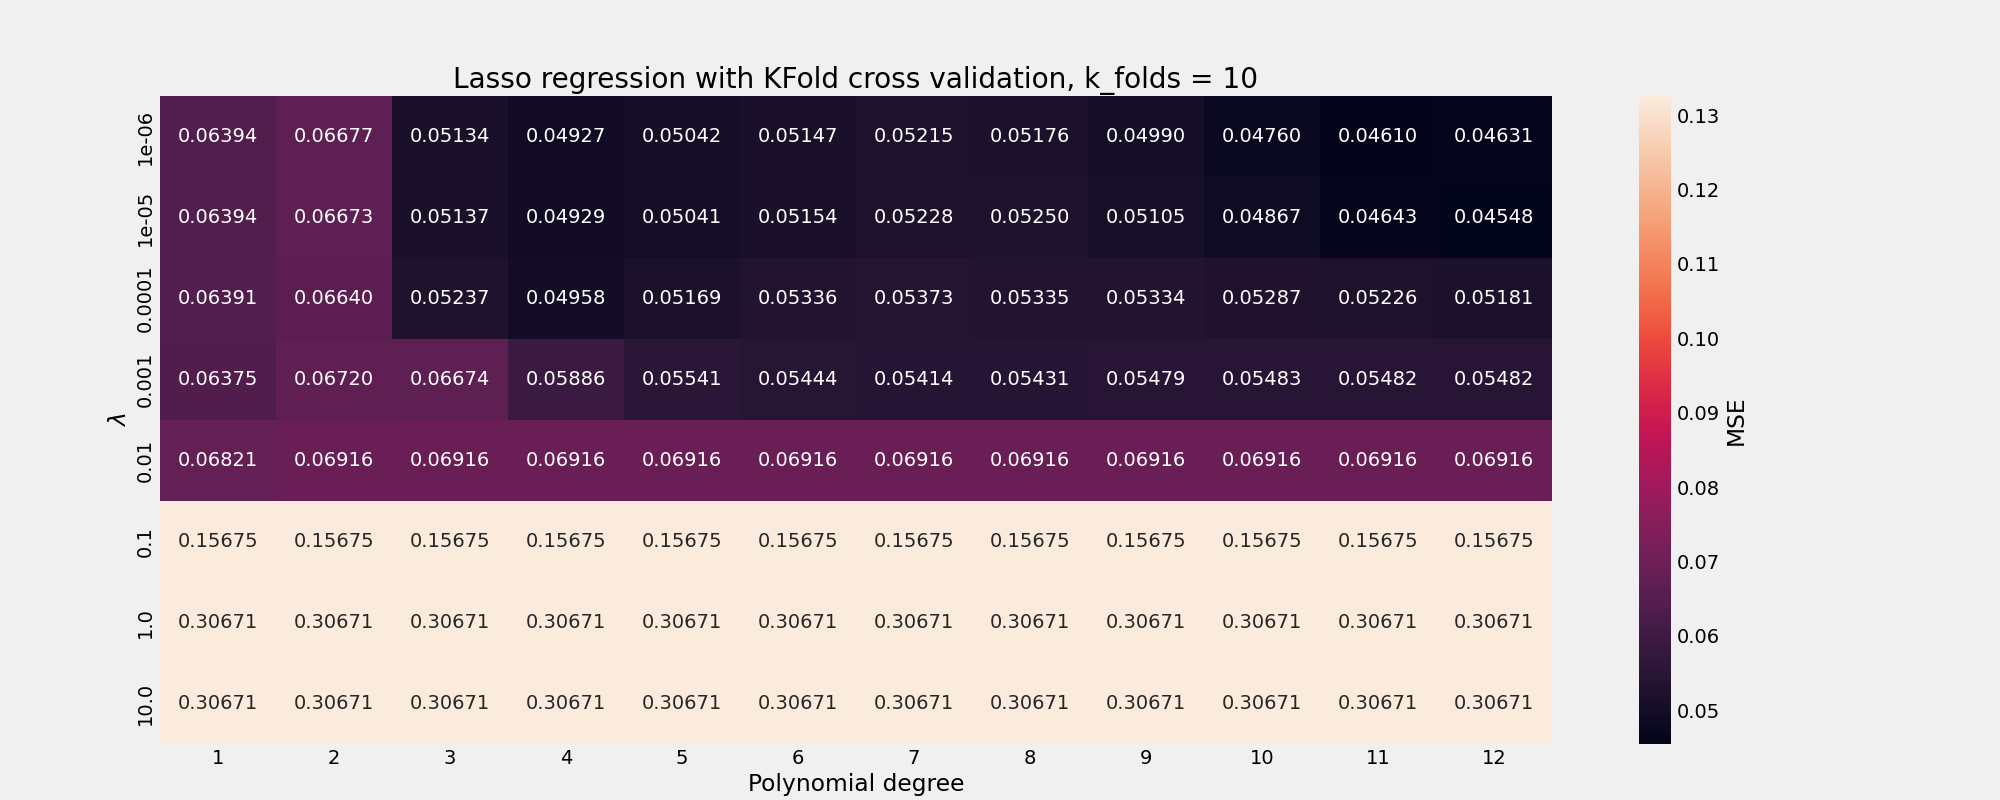
\includegraphics[width=0.8\textwidth]{Figures/f_lasso_kfold_n_10.png}
\end{figure}



% TODO: comparison of MSE for all methods
 
 %Maybe split results into two parts, Franke and Terrain data

%According to red line in report we want:
%On Franke-Function
%Subplot of MSE and R^2, test and training data, for OLS
%Subplot of MSE and R^2, test and training data, for Lasso
%Subplot of MSE and R^2, test and training data, for Ridge
%Comparrison of Regression methods
%Beta plot, but how to do this nicely, to show how beta values get large when polynomial degree increases.
%Resampling: bias-variance plot of bootstrap and cross-validation
%Study lambda dependence (correlation plot)

%On Terrain-data
%Subplot of MSE and R^2, test and training data, for OLS
%Subplot of MSE and R^2, test and training data, for Lasso
%Subplot of MSE and R^2, test and training data, for Ridge
%Comparrison of Regression methods
%Resampling: bias-variance plot of bootstrap and cross-validation
%Study lambda dependence (correlation plot)

%For critical discussion of centering/scaling, from lecture notes: "If our predictors represent different scales, then it is important to standardize the design matrix  by subtracting the mean of each column from the corresponding column and dividing the column with its standard deviation."

%Small test here

\begin{figure}
     \centering
     \begin{subfigure}[b]{0.5\textwidth}
         \centering
         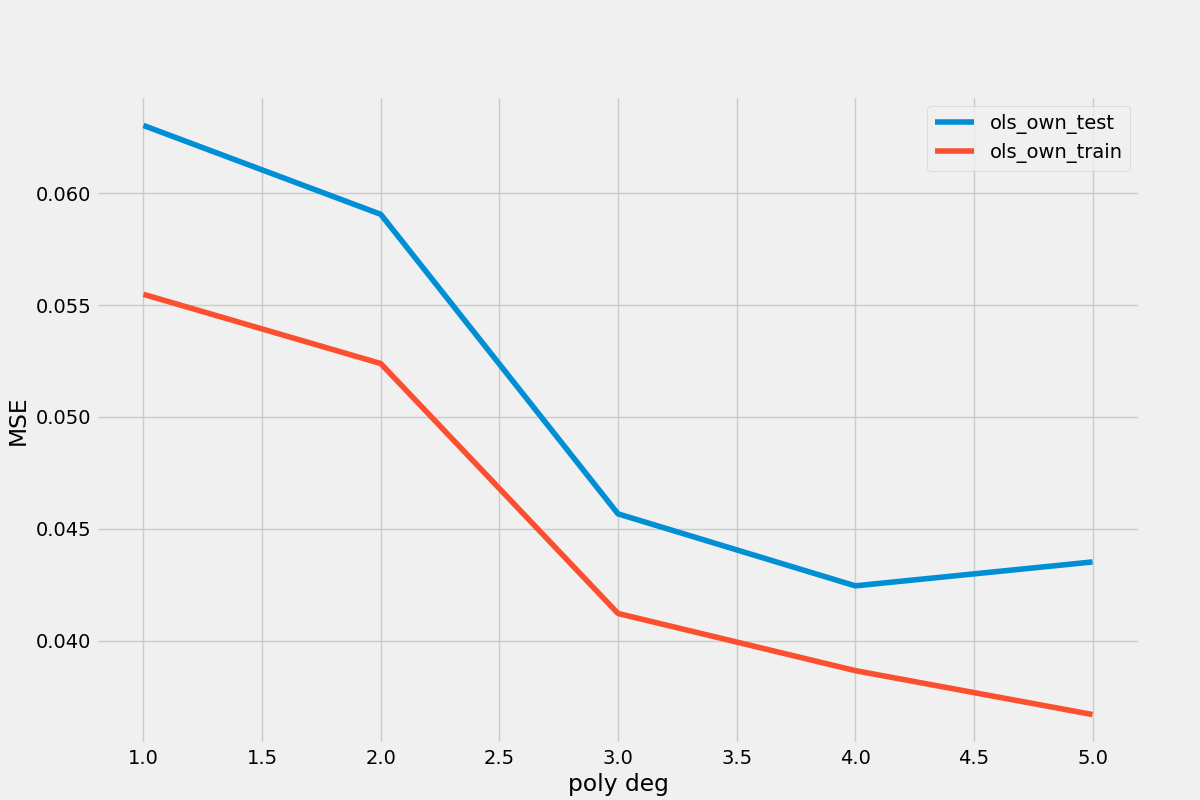
\includegraphics[width=\textwidth]{Figures/b_mse.png}
         \caption{}
         \label{fig:}
     \end{subfigure}%
     \hfill
     \begin{subfigure}[b]{0.5\textwidth}
         \centering
         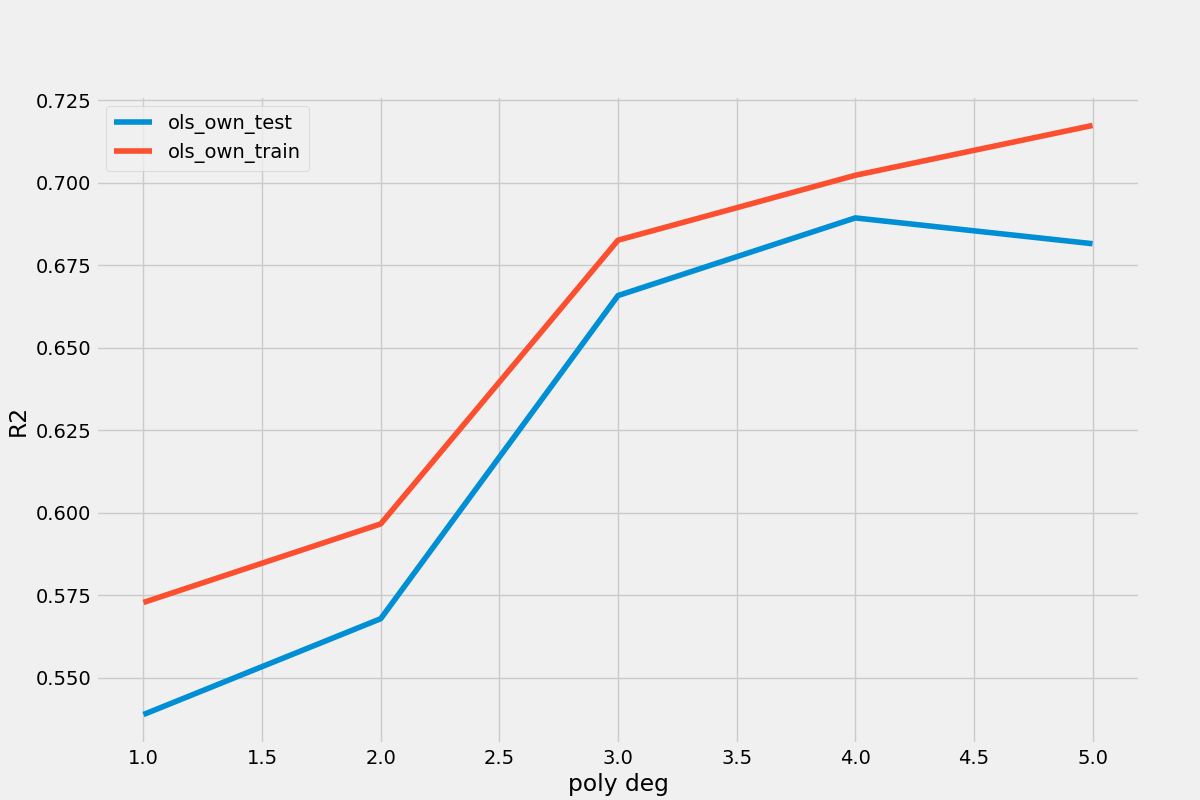
\includegraphics[width=\textwidth]{Figures/b_r2.png}
         \caption{}
         \label{fig:}
     \end{subfigure}
        \caption{Mean squared error and score function for the Ordinary Least Squares (OLS) method. }
        \label{fig:}
\end{figure}






